% arara: pdflatex
% arara: biber
% arara: pdflatex

\documentclass[a4paper]{article}
\usepackage[lighttt]{lmodern}
\ttfamily

% this is to fix a bug in the lmodern
\DeclareFontShape{OT1}{lmtt}{m}{it}
     {<->sub*lmtt/m/sl}{}
     
\usepackage[toc,page]{appendix}
%\usepackage{wrapfig}
\usepackage[pdftex]{graphicx}
%\usepackage[version=3]{mhchem}
\usepackage{fancyvrb}
%\usepackage{multirow}
\usepackage{url}
\usepackage{amsmath}
\usepackage{amssymb}
%package for this is ``algorithms''
\usepackage{algorithmic}
\usepackage{algorithm}
\usepackage{framed}

% this uses the IEEE naming conventions (apart from Procedure)
% \floatname{algorithm}{Procedure}
\renewcommand{\algorithmicrequire}{\textbf{Input:}}
\renewcommand{\algorithmicensure}{\textbf{Output:}}

% Making appendix work as part.
\usepackage{bookmark}


%\usepackage{threeparttable}
\author{Jim Finnis}

\newcommand{\todo}[1]{
    \begin{center}
    \fbox{\parbox{4in}{\textbf{To Do}\vspace*{1em} \\#1}}
    \end{center}}

\newenvironment{important}
{\begin{quote}\color{red}\large%
\begin{center}{\Large \textbf{IMPORTANT}}\end{center}}
{\end{quote}}

\newenvironment{todoblock}
{\begin{quote}\color{red}\large%
\begin{center}{\Large \textbf{ToDo}}\end{center}}
{\end{quote}}

\newenvironment{notebox}[1][]
{\begin{framed}%
\ifthenelse{\equal{#1}{}}{}{%
    \begin{center}%
    {\Large \textbf{#1}}%
    \end{center}%
    }%
    }%    
{\end{framed}}


\DeclareMathOperator*{\argmin}{arg\,min}
\DeclareMathOperator*{\argmax}{arg\,max}
%\DeclareMathOperator*{\max}{arg\,max}
%\DeclareMathOperator*{\min}{arg\,max}
\DeclareMathOperator{\rand}{rand}
                                                                                           
% different commands for left and right margin notes                                                                                                   
\newcommand{\weeboxL}[1]{\rule{15mm}{0.5pt}\\ \parbox[t]{15mm}{\raggedright\footnotesize#1}}                                                                         
\newcommand{\weeboxR}[1]{\rule{15mm}{0.5pt}\\ \parbox[t]{15mm}{\raggedleft\footnotesize#1}}
                                                                                                                                                       
% this selects which command to use for margin notes                                                                                                   
\newcommand{\marg}[1]{\marginpar[\weeboxL{#1}]{\weeboxR{#1}}}

%\newcommand{\marg}[1]{\marginpar{\raggedright\footnotesize #1}}

% In math mode, put a word into text inside anglebrackets. Used for BNF, sometimes.
\newcommand{\angb}[1]{\text{$<$\\#1$>$}}

% so we can do 3\e{4} to do 3x10^4
\providecommand{\e}[1]{\ensuremath{\times 10^{#1}}}

\newenvironment{idescription}%
  {\begin{list}{}{\setlength{\labelwidth}{-10pt}
   \setlength{\itemindent}{-\leftmargin}
   \setlength{\listparindent}{\parindent}
   \renewcommand{\makelabel}{\descriptionlabel}}}%
  {\end{list}}


\DefineVerbatimEnvironment{v}{Verbatim}{
    %numbers=left,numbersep=5pt,
    %frame=lines,framerule=0.5mm,
    fontsize=\small,xleftmargin=15pt}
\DefineVerbatimEnvironment{vv}{Verbatim}{
    %numbers=left,numbersep=5pt,
    %frame=lines,framerule=0.5mm,
    fontsize=\small,xleftmargin=15pt}
\DefineVerbatimEnvironment{v2}{Verbatim}{
    %numbers=left,numbersep=5pt,
    %frame=lines,framerule=0.5mm,
    fontsize=\scriptsize,xleftmargin=0pt}
\DefineVerbatimEnvironment{v3}{Verbatim}{
    %numbers=left,numbersep=5pt,
    %frame=lines,framerule=0.5mm,
    fontsize=\tiny,xleftmargin=0pt}
\DefineVerbatimEnvironment{bv2}{BVerbatim}{
    %numbers=left,numbersep=5pt,
    %frame=lines,framerule=0.5mm,
    fontsize=\scriptsize,xleftmargin=0pt}
\DefineVerbatimEnvironment{bv}{BVerbatim}{
    %numbers=left,numbersep=5pt,
    %frame=lines,framerule=0.5mm,
    fontsize=\scriptsize,xleftmargin=0pt}
\DefineVerbatimEnvironment{bvc}{BVerbatim}{
    %numbers=left,numbersep=5pt,
    %frame=lines,framerule=0.5mm
    commandchars=+\[\],
    fontsize=\scriptsize,xleftmargin=0pt}

\setcounter{secnumdepth}{5}
\setcounter{tocdepth}{5}

%\usepackage[hmargin=2.5cm,vmargin=3.5cm]{geometry}
\usepackage[hmargin=3cm,
    vmargin=5cm,
    marginparwidth=2.0cm,
    ]{geometry}
\usepackage{multicol}
\usepackage{caption}
\usepackage{subcaption}
\usepackage{booktabs}
\usepackage{boldline}
\usepackage{multirow}
\usepackage{pdflscape}
\usepackage{afterpage}
\usepackage{amsmath}
\usepackage[all]{xy}
\usepackage{letltxmacro}
% uncomment this to enable internal automatic hyperlinks
\usepackage{hyperref}
\hypersetup{colorlinks}
\usepackage{listings}
\usepackage[usenames,dvipsnames]{color}
%Citation uses biber, and we set the style here
\usepackage[backend=biber,style=numeric,url=false]{biblatex}

\addbibresource{bib.bib}
\usepackage[font=small,labelfont=bf,margin=3em]{caption}
%\usepackage[LGR,T1]{fontenc}
%\newcommand{\textgreek}[1]{\begingroup\fontencoding{LGR}\selectfont#1\endgroup}
\usepackage{tikz}
%\usetikzlibrary{positioning}
\lstdefinelanguage{angort}{
morekeywords={for,if,then,else,leave,dup,call,global,swap,drop,not,
and,or,ifleave,const,over,defer,each,include,stop,dumplist,get,set,len,remove,shift,unshift,pop,push,map,reduce,filter,in,version,
barewords,dump,snark,none,p,x,rawp,nl,quit,debug,disasm,assertdebug,assert,assertmode,
abs,neg,isnone,gccount,range,srange,frange,frangesteps,i,j,k,iter,save,load,clear,
list,help,type,srand,rand,gc,format},
sensitive=false,
morecomment=[l]{\#},
morestring=[b]"
}
\lstdefinestyle{Python}{
  belowcaptionskip=1\baselineskip,
  breaklines=true,
  frame=L,
  xleftmargin=\parindent,
  language=Python,
  showstringspaces=false,
  basicstyle=\ttfamily\scriptsize,
  stringstyle=\slshape,
}
% patch fullcite to include the citation key
\LetLtxMacro\oldfullcite\fullcite
\renewcommand{\fullcite}[1]{\cite{#1}: \oldfullcite{#1}}

% This is a command to do subfigures easily. It's based on a
% stackoverflow hack : http://tex.stackexchange.com/questions/72902/new-command-with-variable-number-of-parameters
% The basic idea:
%
% The macro \twoimages really has no argument; it simply starts the
% business by opening the figure environment and calls the real command,
% \@twoimagesi. This command checks whether it's followed by
% \stopimages; if it is, it calls \@twoimagesend that ends the
% environment; otherwise it executes \@twoimagesii that has the job of
% printing a row, after having absorbed its six arguments. It does so in
% an indirect way, so that we can write only once the same minipage,
% using the first three arguments and the last three.
% Then \@twoimagesii restarts the recursion by calling \@twoimagesi again.
%
% Usage:
% \twoimages{caption}{label}
% {filename}{subcaption}
% {filename}{subcaption}
% {filename}{subcaption}
% \stopimages
%
% Labels will also be generated for each image, which are the filenames
% of the images.
%
% Optional command for image size multiplier

\makeatletter % we need to use kernel commands
\newcommand{\twoimages}[3][1]{%
  \def\jcf@tmpsiz{#1}
  \def\jcf@tmpcap{#2}
  \def\jcf@tmplab{#3}
  \begin{figure}[!htb]
  \@twoimagesi
}
\newcommand\@twoimagesi{\@ifnextchar\stopimages{\@twoimagesend}{\@twoimagesii}}

\newcommand\@twoimagesii[4]{%
  \@twoimagesiii{#1}{#2}\hfill
  \@twoimagesiii{#3}{#4}\\[\bigskipamount]
  \@twoimagesi % restart the recursion
}
\newcommand\@twoimagesiii[2]{%
  \begin{subfigure}{0.49\linewidth}
    \centering
    \includegraphics[width=\jcf@tmpsiz\textwidth]{#1}
    \caption{#2}\label{#1}
  \end{subfigure}}
\newcommand\@twoimagesend[1]{% The argument is \stopimages
  \vspace*{-\bigskipamount}
  \caption{\jcf@tmpcap \textit{(Label: \jcf@tmplab)}}\label{\jcf@tmplab}
  \end{figure}}
\makeatother

% similar but each line also takes a label
\makeatletter % we need to use kernel commands
\newcommand{\twoimageslabel}[3][1]{%
  \def\jcf@tmpsiz{#1}
  \def\jcf@tmpcap{#2}
  \def\jcf@tmplab{#3}
  \begin{figure}[!htb]
  \@twoimageslabeli
}
\newcommand\@twoimageslabeli{\@ifnextchar\stopimages{\@twoimageslabelend}{\@twoimageslabelii}}

\newcommand\@twoimageslabelii[6]{%
  \@twoimageslabeliii{#1}{#2}{#3}\hfill
  \@twoimageslabeliii{#4}{#5}{#6}\\[\bigskipamount]
  \@twoimageslabeli % restart the recursion
}
\newcommand\@twoimageslabeliii[3]{%
  \begin{subfigure}{0.49\linewidth}
    \centering
    \includegraphics[width=\jcf@tmpsiz\textwidth]{#1}
    \caption{#2}\label{#3}
  \end{subfigure}}
\newcommand\@twoimageslabelend[1]{% The argument is \stopimages
  \vspace*{-\bigskipamount}
  \caption{\jcf@tmpcap \textit{(Label: \jcf@tmplab)}}\label{\jcf@tmplab}
  \end{figure}}
\makeatother

% similar but each line is unlabelled
\makeatletter % we need to use kernel commands
\newcommand{\twoimagesnolabel}[3][1]{%
  \def\jcf@tmpsiz{#1}
  \def\jcf@tmpcap{#2}
  \def\jcf@tmplab{#3}
  \begin{figure}[!htb]
  \@twoimagesnolabeli
}
\newcommand\@twoimagesnolabeli{\@ifnextchar\stopimages{\@twoimagesnolabelend}{\@twoimagesnolabelii}}

\newcommand\@twoimagesnolabelii[4]{%
  \@twoimagesnolabeliii{#1}{#2}\hfill
  \@twoimagesnolabeliii{#3}{#4}\\[\bigskipamount]
  \@twoimagesnolabeli % restart the recursion
}
\newcommand\@twoimagesnolabeliii[2]{%
  \begin{subfigure}{0.49\linewidth}
    \centering
    \includegraphics[width=\jcf@tmpsiz\textwidth]{#1}
    \caption{#2}
  \end{subfigure}}
\newcommand\@twoimagesnolabelend[1]{% The argument is \stopimages
  \vspace*{-\bigskipamount}
  \caption{\jcf@tmpcap \textit{(Label: \jcf@tmplab)}}\label{\jcf@tmplab}
  \end{figure}}
\makeatother


% similar, but for three parallel images. More is just silly.


\makeatletter % we need to use kernel commands
\newcommand{\threeimages}[2]{%
  \def\jcf@tmpcap{#1}
  \def\jcf@tmplab{#2}
  \begin{figure}[!htb]
  \@threeimagesi
}
\newcommand\@threeimagesi{\@ifnextchar\stopimages{\@threeimagesend}{\@threeimagesii}}

\newcommand\@threeimagesii[6]{%
  \@threeimagesiii{#1}{#2}\hfill
  \@threeimagesiii{#3}{#4}\hfill
  \@threeimagesiii{#5}{#6}\\[\bigskipamount]
  \@threeimagesi % restart the recursion
}
\newcommand\@threeimagesiii[2]{%
  \begin{subfigure}{0.33\linewidth}
    \centering
    \includegraphics[width=\textwidth]{#1}
    \caption{#2}\label{#1}
  \end{subfigure}}
\newcommand\@threeimagesend[1]{% The argument is \stopimages
  \vspace*{-\bigskipamount}
  \caption{\jcf@tmpcap \textit{(Label: \jcf@tmplab)}}\label{\jcf@tmplab}
  \end{figure}}
\makeatother


% similar but takes any number of images and just puts them on subsequent lines at a given
% scale of the linewidth (the third argument).

\makeatletter % we need to use kernel commands
\newcommand{\multiimages}[3]{%
  \def\jcf@tmpcap{#1}
  \def\jcf@tmplab{#2}
  \def\jcf@tmpwidth{#3}
  \begin{figure}[!htb]
  \@multiimagesi
}
\newcommand\@multiimagesi{\@ifnextchar\stopimages{\@multiimagesend}{\@multiimagesii}}

\newcommand\@multiimagesii[2]{%
  \@multiimagesiii{#1}{#2} \\[\bigskipamount]
  \@multiimagesi % restart the recursion
}
\newcommand\@multiimagesiii[2]{%
  \begin{subfigure}{\linewidth}
    \centering
    \includegraphics[width=\jcf@tmpwidth\textwidth]{#1}
    \caption{#2}\label{#1}
  \end{subfigure}}
\newcommand\@multiimagesend[1]{% The argument is \stopimages
  \vspace*{-\bigskipamount}
  \caption{\jcf@tmpcap \textit{(Label: \jcf@tmplab)}}\label{\jcf@tmplab}
  \end{figure}}
\makeatother

% permits equation numbering in starred environments, so we can then
% label with \numberthis\label..

\newcommand\numberthis{\addtocounter{equation}{1}\tag{\theequation}}


\title{PCOT design notes}
\author{James Finnis (jcf12@aber.ac.uk)}

\begin{document}
\lstset{style=Python}
\maketitle
\LetLtxMacro\oldincludegraphics\includegraphics
% Stuff to redefine includegraphics to show the document file
% underneath; useful for referencing.
\renewcommand{\includegraphics}[2][]{%
%    \rotatebox[origin=tr]{270}{\tiny #2} %
    \oldincludegraphics[#1]{#2}%
    \\{\scriptsize #2}%
}



%Why is this even here?
%\nobibliography*
\tableofcontents


% Created by Jim Finnis
% Date Wed Feb 24 13:35:30 2021


\section{Introduction}
These notes provide some architectural details for PCOT to help
maintainers. I'll try to keep them up to date.

PCOT is based around a directed graph of nodes which perform
transformations of data. For this reason, the nodes are sometimes
called ``transforms'' and are represented by the \texttt{XForm} class
in the code.
Usually the data in question is an image, or rather an ``image cube'':
these have an arbitrary number of channels, not just the typical
RGB or greyscale. However, the data can be anything at all --- it depends
on the node. There is some typechecking when constructing the graph:
for exampel, you can't connect a ``rectangle'' output to an ``image'' input.
The entire application is shown in Fig.~\ref{app.png}. On the right
is a ``palette'' from which nodes can be selected to add to the graph,
while on the left
is an area which can show controls for each node in the graph, while
in the centre-right is the graph itself. This is shown in more detail
in Fig.~\ref{graph.png}.

\begin{figure}[ht]
\center
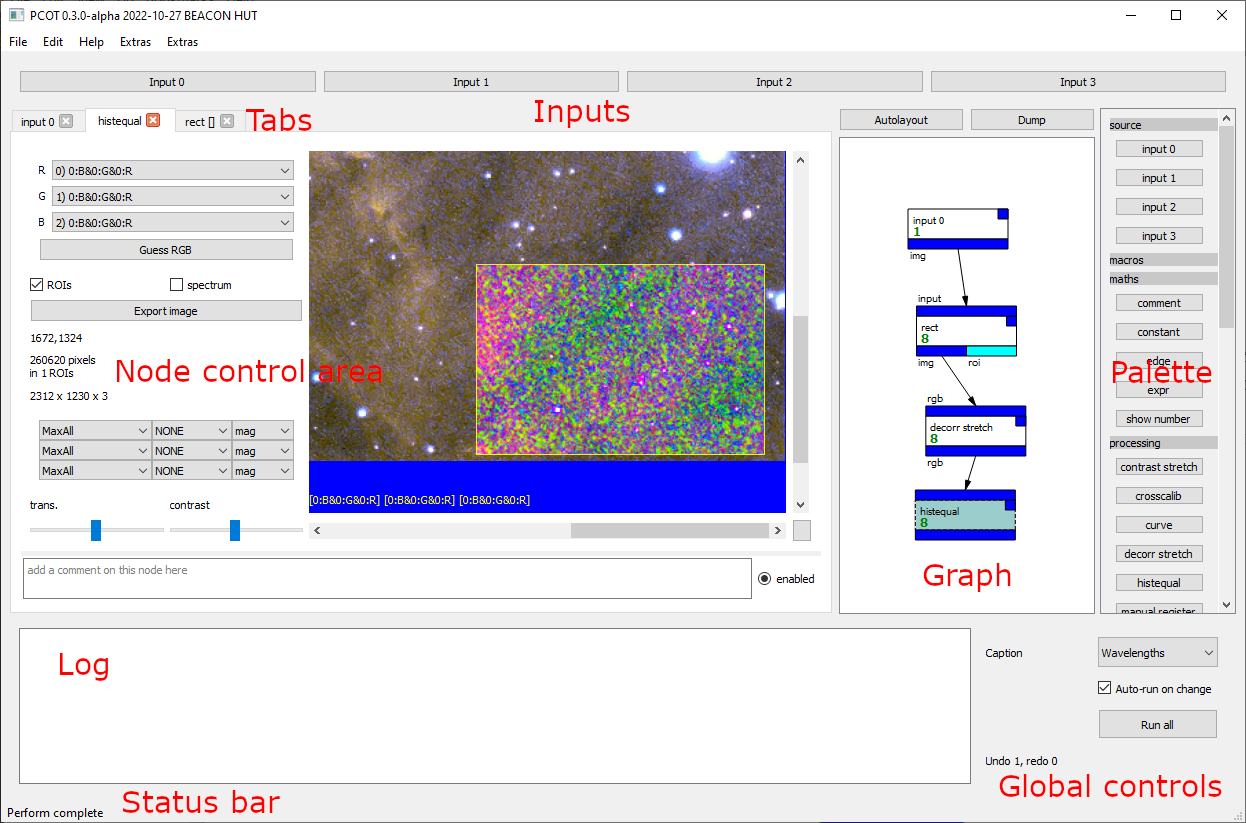
\includegraphics[width=6in]{app.png}
\caption{The PCOT application}
\label{app.png}
\end{figure}

\clearpage This will take an image from one of the data inputs --- these
exist independently of the graph proper and are configured with the four buttons
at the top of the window, see Sec.~\ref{inputs} ---
and perform a decorrelation stretch followed by a histogram
equalisation on the three channels selected in the \texttt{rect} node.
It will only do this to a rectangular
portion of the image (defined by the \texttt{rect} node), annotating the
region with some text defined in that node's controls. The
control region is currently showing the output of the histogram equalisation.

\begin{figure}[ht]
\center
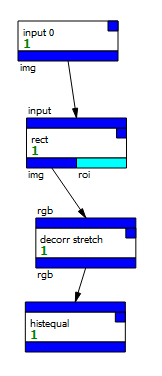
\includegraphics[width=1.4in]{graph.png}
\caption{An example graph}
\label{graph.png}
\end{figure}


\subsection{Notes on type checking}
Python is dynamically typed, but there are a lot of ``type annotations''
in the code. Unfortunately, Python's import rules mean there's also some
odd stuff going on. Annotations like
\begin{lstlisting}
class XFormType:
    ## @var name
    # name of the type
    name: str
    ## @var group
    # the palette group to which it belongs
    group: str
    ## @var ver
    # version number
    ver: str
    ## @var hasEnable
    # does it have an enable button?
\end{lstlisting}
are straightforward (and note the Doxygen annotations): we have three
string fields (\texttt{name}, \texttt{group} and \texttt{ver}) and
a boolean field (\texttt{hasEnable}). The next annotation, however,
is a link to a class defined further down the file, which in turn has
a field which is \texttt{XFormType}: a cyclic dependency. In such cases,
the standard PEP 0484 tactic is to use a string literal --- the type
checker will resolve this successfully and give appropriate warnings:
\begin{lstlisting}
    ## @var instances
    # all instances of this type in all graphs
    instances: List['XForm']
\end{lstlisting}
defines \texttt{instances} as a list of \texttt{XForm}.

Another oddity you may see in some of the files is this (from the top
of \texttt{xform.py} like the previous example):
\begin{lstlisting}
if TYPE_CHECKING:
    import graphscene
    import PyQt5.QtWidgets
\end{lstlisting}
These lines are only run when type checking, and are used to ensure
that appropriate classes are imported for type hints like this:
\begin{lstlisting}
    ## @var rect
    # the main rectangle for the node in the scene
    rect: ['graphscene.GMainRect']
    ## @var inrects
    # input connector rectangles
    inrects: List[Optional['graphscene.GConnectRect']]
    ## @var outrects
    # output connector rectangles
    outrects: List[Optional['graphscene.GConnectRect']]
    ## @var helpwin
    # an open help window, or None
    helpwin: Optional['PyQt5.QtWidgets.QMainWindow']
\end{lstlisting}
Without the \texttt{TYPE\_CHECKING} guard the program will not run, because
these imports are actually cyclic. However, they are only needed at 
compile time, so the \texttt{if}-statement is added to stop the import
at run time. Note the quotes: they are there to stop Python trying to
resolve the symbols at run time.


% Created by Jim Finnis
% Date Wed Feb 24 13:48:57 2021


\section{The data model}
The data model consists of two parts --- the data itself (largely
image cube data) and the graph. By far the most important kind of data
from the point of view of this document is the image data, which ties
into the user interface in complex ways. Other forms of data do exist,
but these are much simpler.


\subsection{Graph and nodes}
The graph is a directed graph of nodes represented by the 
\texttt{XFormGraph} class. Each node is an instance of \texttt{XForm}
(short for ``transform node''). The function of each node is
determined by its \texttt{type} field, which references an
\texttt{XFormType} singleton. See Fig.~\ref{xform.pdf} for an overview.

\begin{figure}[ht]
\center
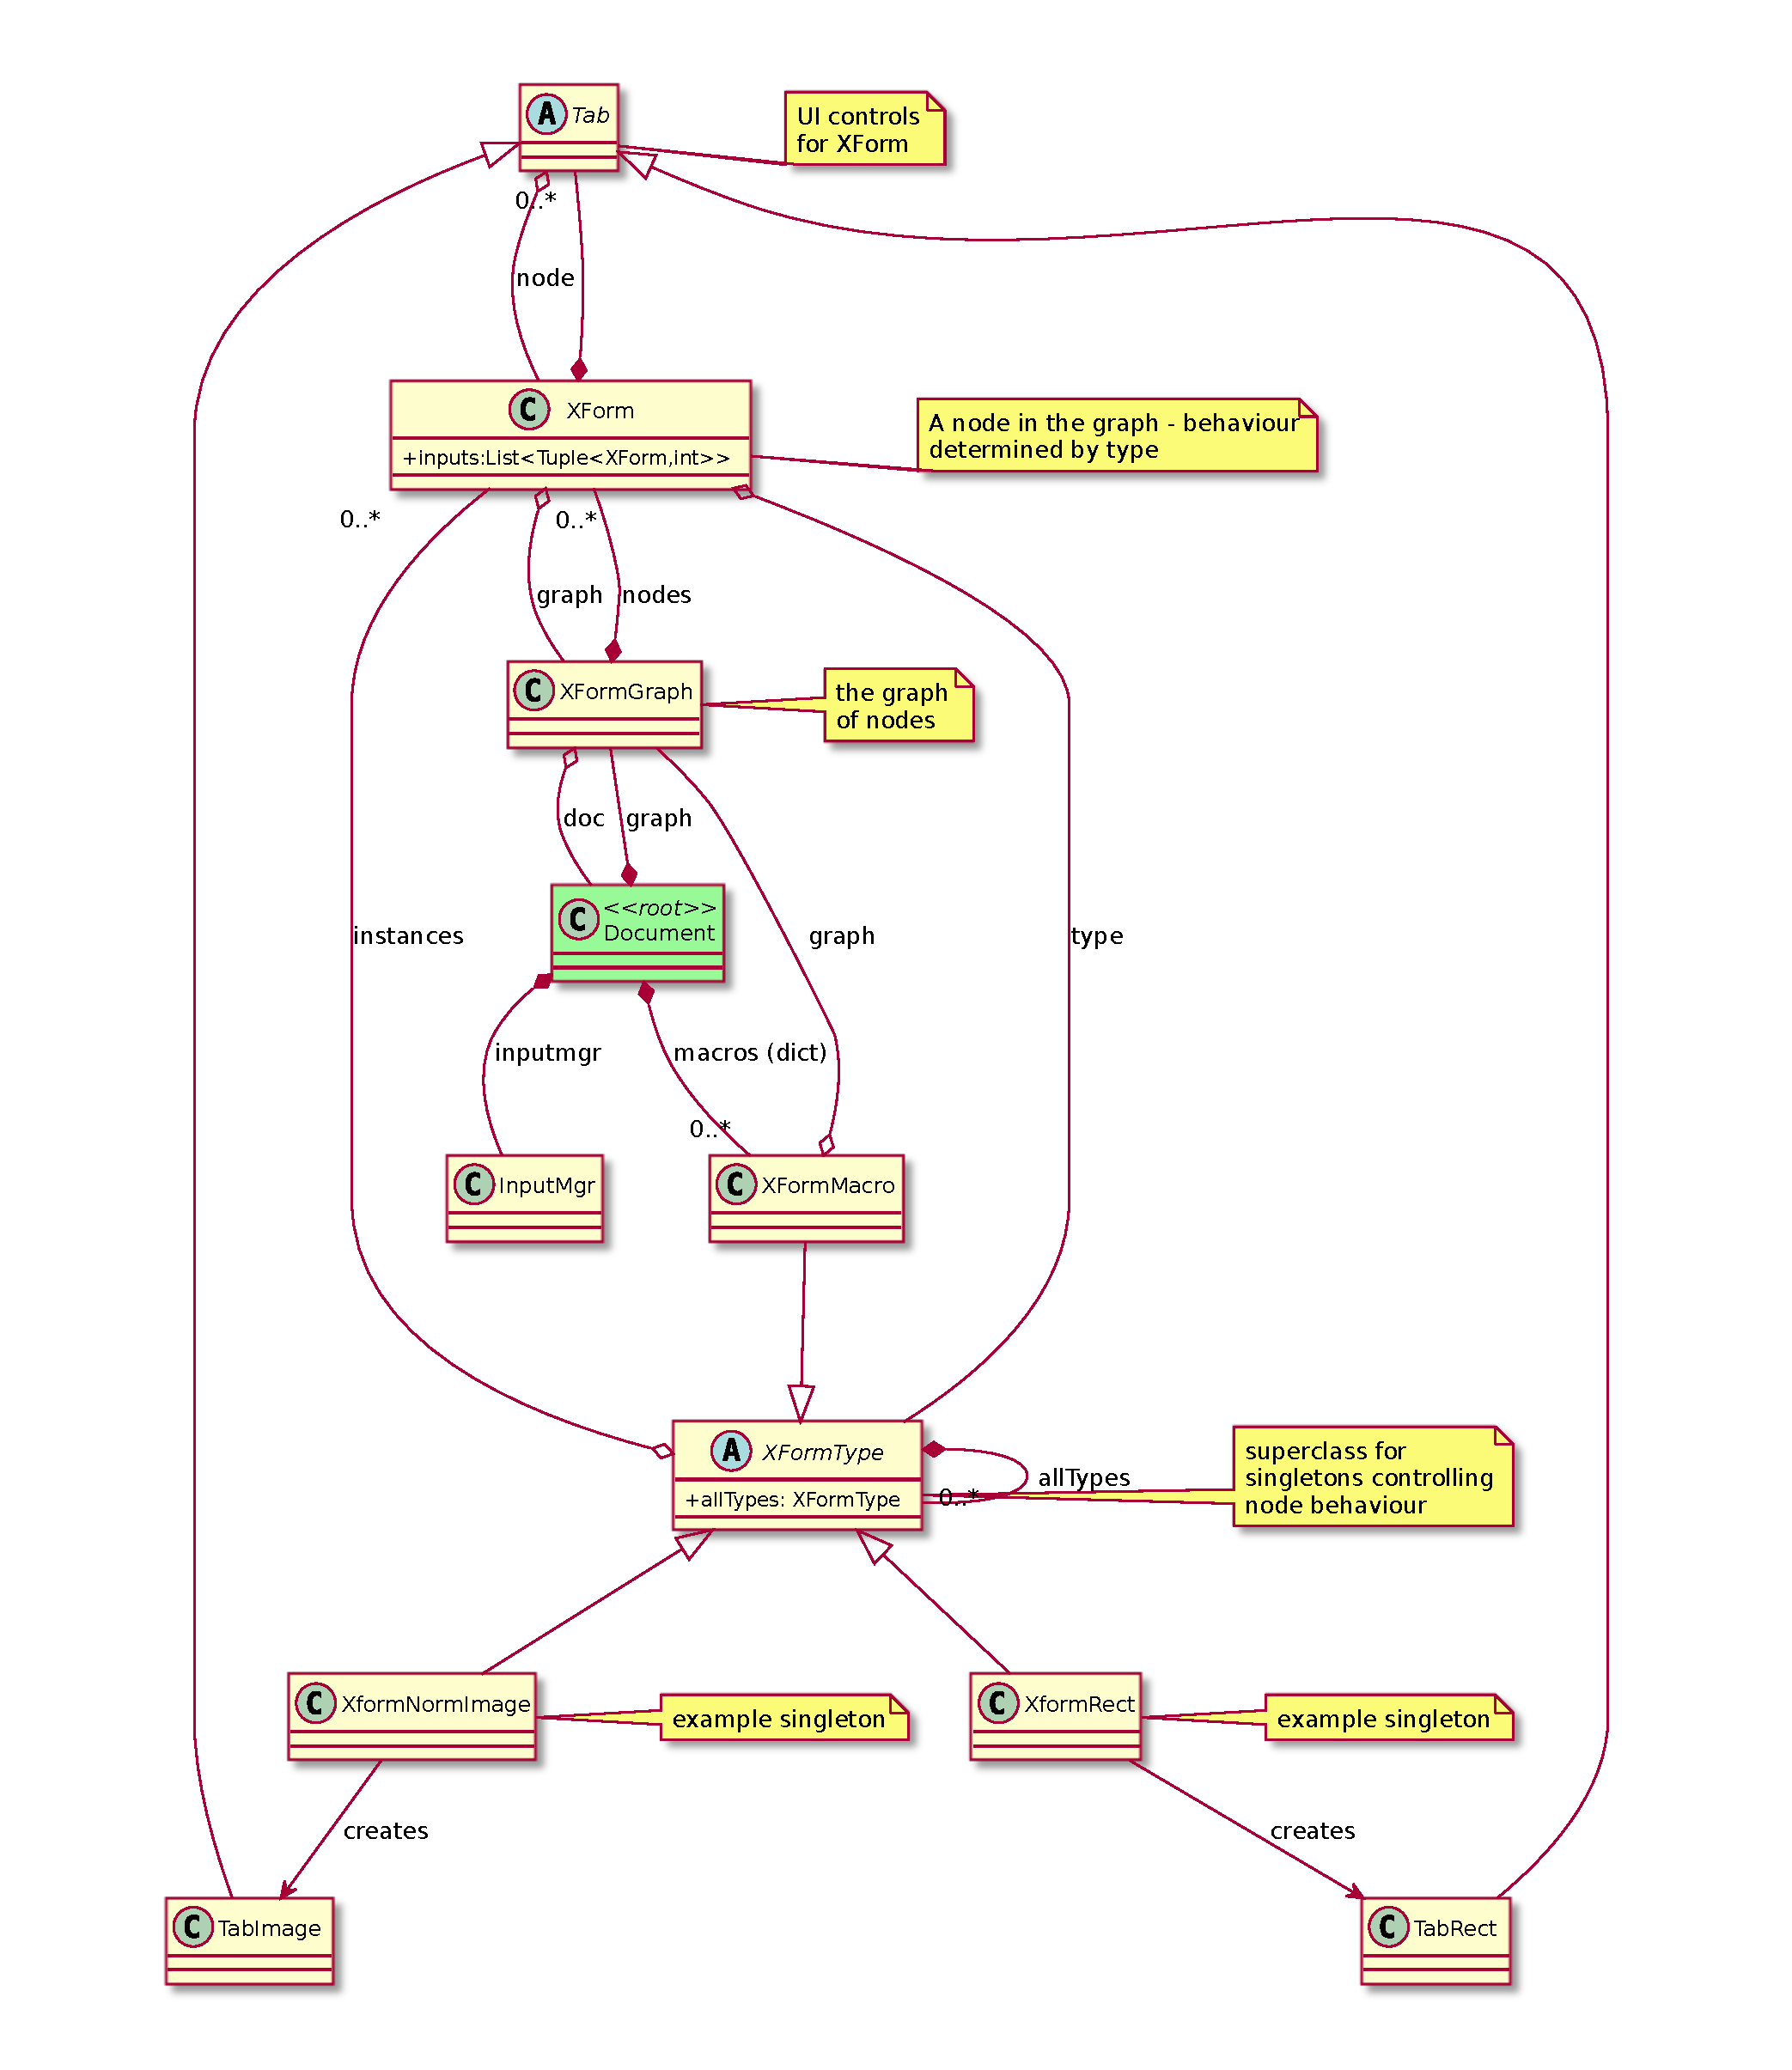
\includegraphics[width=5in]{xform.pdf}
\caption{\texttt{XForm} and graph model}
\label{xform.pdf}
\end{figure}

\subsubsection{XFormType and type registration}
\label{xformtype}
Each node type is represented by a subclass of \texttt{XFormType},
and each subclass has a singleton to which nodes of that type link.
For example, the \emph{rect} node's behaviour is specified by
the \texttt{XformRect} class, which has a singleton instance. All
\texttt{XForm} nodes which are \emph{rect} nodes have a \texttt{type} field
pointing to this singleton.

The singletons are automatically created and registered when the class
is defined, through the \texttt{@xformtype} decorator. This does the
following:
\begin{itemize}
\item Creates an instance of the class;
\item Creates an MD5 hash of the class' source code which is stored
inside the type singleton for version control;
\item Changes the semantics of the class constructor so that
it always returns the instance we just created (thus making the class
a singleton).
\end{itemize}
The base constructor for \texttt{XFormType} adds the singleton
to a dictionary class variable \texttt{allTypes}, so we can always
obtain the singleton object and create new nodes which perform that
node type.

\subsubsection{XFormType methods}
In order to perform a node's action, the type classes must contain
the following methods:
\begin{itemize}
\item \texttt{init(node:XForm)} : initialise any extra data inside
the node required to perform this type's behaviour
\item \texttt{perform(node:XForm)} : perform this node's behaviour ---
read any inputs, manipulate the data, set the outputs.
\item \texttt{createTab(node:XForm, window:MainWindow)} : create a UI tab to edit/view this node.
\end{itemize}
Several other methods may optionally be overridden.

\subsubsection{Linkage}
\texttt{XForm} node objects are linked together by their inputs.
Each \texttt{XForm} contains an \texttt{inputs} list indexed by
input number. The length of this list is determined by the number
of inputs the type object specifies. Each entry is a $(node,output)$
tuple where $node$ is a reference to another \texttt{XForm} and
$output$ is the index of an output on that \texttt{XForm}.

Methods are provided in \texttt{XForm} for connecting and disconnecting nodes
(also checking for cycles and providing basic type checking), and getting inputs
and setting outputs inside the type's \texttt{perform()} method.

The number and types of inputs and outputs is set inside the 
constructor for the \texttt{XFormType} singleton, by using methods
to add these connectors. They are then indexed in order of creation.
For example, the \emph{inset} \texttt{XFormType} has the constructor:
\begin{lstlisting}
    def __init__(self):
        super().__init__("inset", "regions", "0.0.0")
        self.addInputConnector("img", "img")        # input 0
        self.addInputConnector("inset", "img")      # input 1
        self.addInputConnector("rect", "rect")      # input 2
        self.addOutputConnector("", "img")
\end{lstlisting}
The arguments for these methods are $(name,type)$ where the name is 
optional (used by the UI to show a hint).

\subsection{Performing the graph}
\label{graphperform}
The graph needs to be ``performed'' --- its nodes executed --- whenever
the data changes, which is generally whenever the graph is edited or
a node control changed in a tab.
This is done by calling \texttt{changed()} on the node's graph.
The \texttt{XFormGraph.changed(node)} method takes a node, and either calls
\texttt{performNodes()} on the main graph passing in that node, or, if the
node is inside a macro prototype graph (q.v.), copies the prototype graph to
all its instances and runs \texttt{performNodes()} for all those instances
(see Sec.~\ref{macroineff} for why this is a problem).

The \texttt{XFormGraph.performNodes(node=None)} method itself takes a single argument and performs
either the entire graph or a portion of the graph starting at a particular node.
If the argument is None, the internal list of all nodes in the graph is traversed looking
for nodes with no inputs and these are performed. If the argument is not None that node
is performed. Nodes are performed by calling their \texttt{perform()} method. This will
recursively run the child nodes, but only when they are ``ready to run''
(all their inputs have been set). 

\clearpage
\subsubsection{Performing a node}
The \texttt{XForm.perform()} method will run a node, and recursively run all child nodes, although
there are some complexities here (mainly to accommodate macros). It will not perform the node if it 
has already run in this call to \texttt{performNodes()} or if it is not ready to run (some inputs do not yet have values):
\begin{algorithmic}
\IF{node has not already run \textbf{and} node is ready to run}
\STATE clear all outputs
\STATE run the node type singleton's \texttt{perform()} method on the node
\STATE mark node as having run
\FORALL{$t$ in open tabs for this node}
\STATE $t$\texttt{.onNodeChanged()}
\ENDFOR
\FORALL{$c$ in child nodes}
\STATE perform node $c$
\ENDFOR
\ENDIF
\end{algorithmic}
A node is ready to run if it has no inputs which do not yet have values set. This is
determined by checking the outputs of the nodes from which the inputs come to see if
they have yet been set with values. The \texttt{performNodes()} method is called from only two places:
\begin{itemize}
\item \texttt{XFormGraph.changed(node)}: when the graph or a node in a graph has been changed. This is the most
frequent call, and is typically called with a node to avoid running the whole graph. The node is passed down into
\texttt{performNodes()}).
\item \texttt{XFormMacro.perform(node)}: when a node which contains a macro instance is being performed (see
Sec.~\ref{macros} for more details).
\end{itemize}
The \texttt{XFormGraph.changed()} method is called from several places:
\begin{itemize}
\item \texttt{XFormGraph.runAll()} : called when a graph is explicitly run.
\item \texttt{XForm.disconnect()} and \texttt{XForm.connect()}: when connections between nodes are made or broken.
\item \texttt{XForm.setEnabled()}: when a node is enabled or disabled.
\item \texttt{Tab.changed()}: when a tab signals that a node it controls has had a parameter change.
\item \texttt{XFormGraph.deserialise()}: when a graph has been loaded.
\end{itemize}

\subsubsection{Error handling}
\label{errorhandling}
Error handling is generally required in three cases:
\begin{itemize}
\item connection type mismatch discovered at connect time,
\item connection type mismatch discovered at perform time,
\item other errors at perform time.
\end{itemize}
The first is dealt with using the connection type system
in \texttt{conntypes.py}: each connection (input and output) has a string
type and the connections must match, or they will not be made. An input
of type ``any'' can accept any type. Additional checks are made to avoid
cycles.

The other types of error are both handled inside the node's \texttt{perform()},
and take two forms:
\begin{itemize}
\item either the type's \texttt{perform()} throws an \texttt{XFormException}, which
is handled by \texttt{XForm.perform},
\item or \texttt{perform()} completes but perhaps shows an empty image,
and calls \texttt{setError(exception)} to set the error state.
\end{itemize}
In both cases \texttt{setError()} will print a message to console and
set an error state in the node. This error state
will have been cleared in all nodes before the graph is performed. A redraw of the
entire graph is done after the graph is performed to
draw those nodes in an error state differently, showing the 
brief error code passed into \texttt{XFormException}. The error
will also be shown in the tab for that node and in its ``help box''
(opened by clicking the box in the corner).

\subsection{Image data}
Most classes making up the image data 
model are declared in the \texttt{pancamimage.py} file, including the main \texttt{ImageCube}
class. Some additional classes describing where images can come from are in \texttt{channelsource.py}.
The model is shown in outline in Fig.~\ref{image.pdf} although some links to channel sources
and mapping from nodes are omitted; these will be explained later.

\begin{figure}[ht]
\center
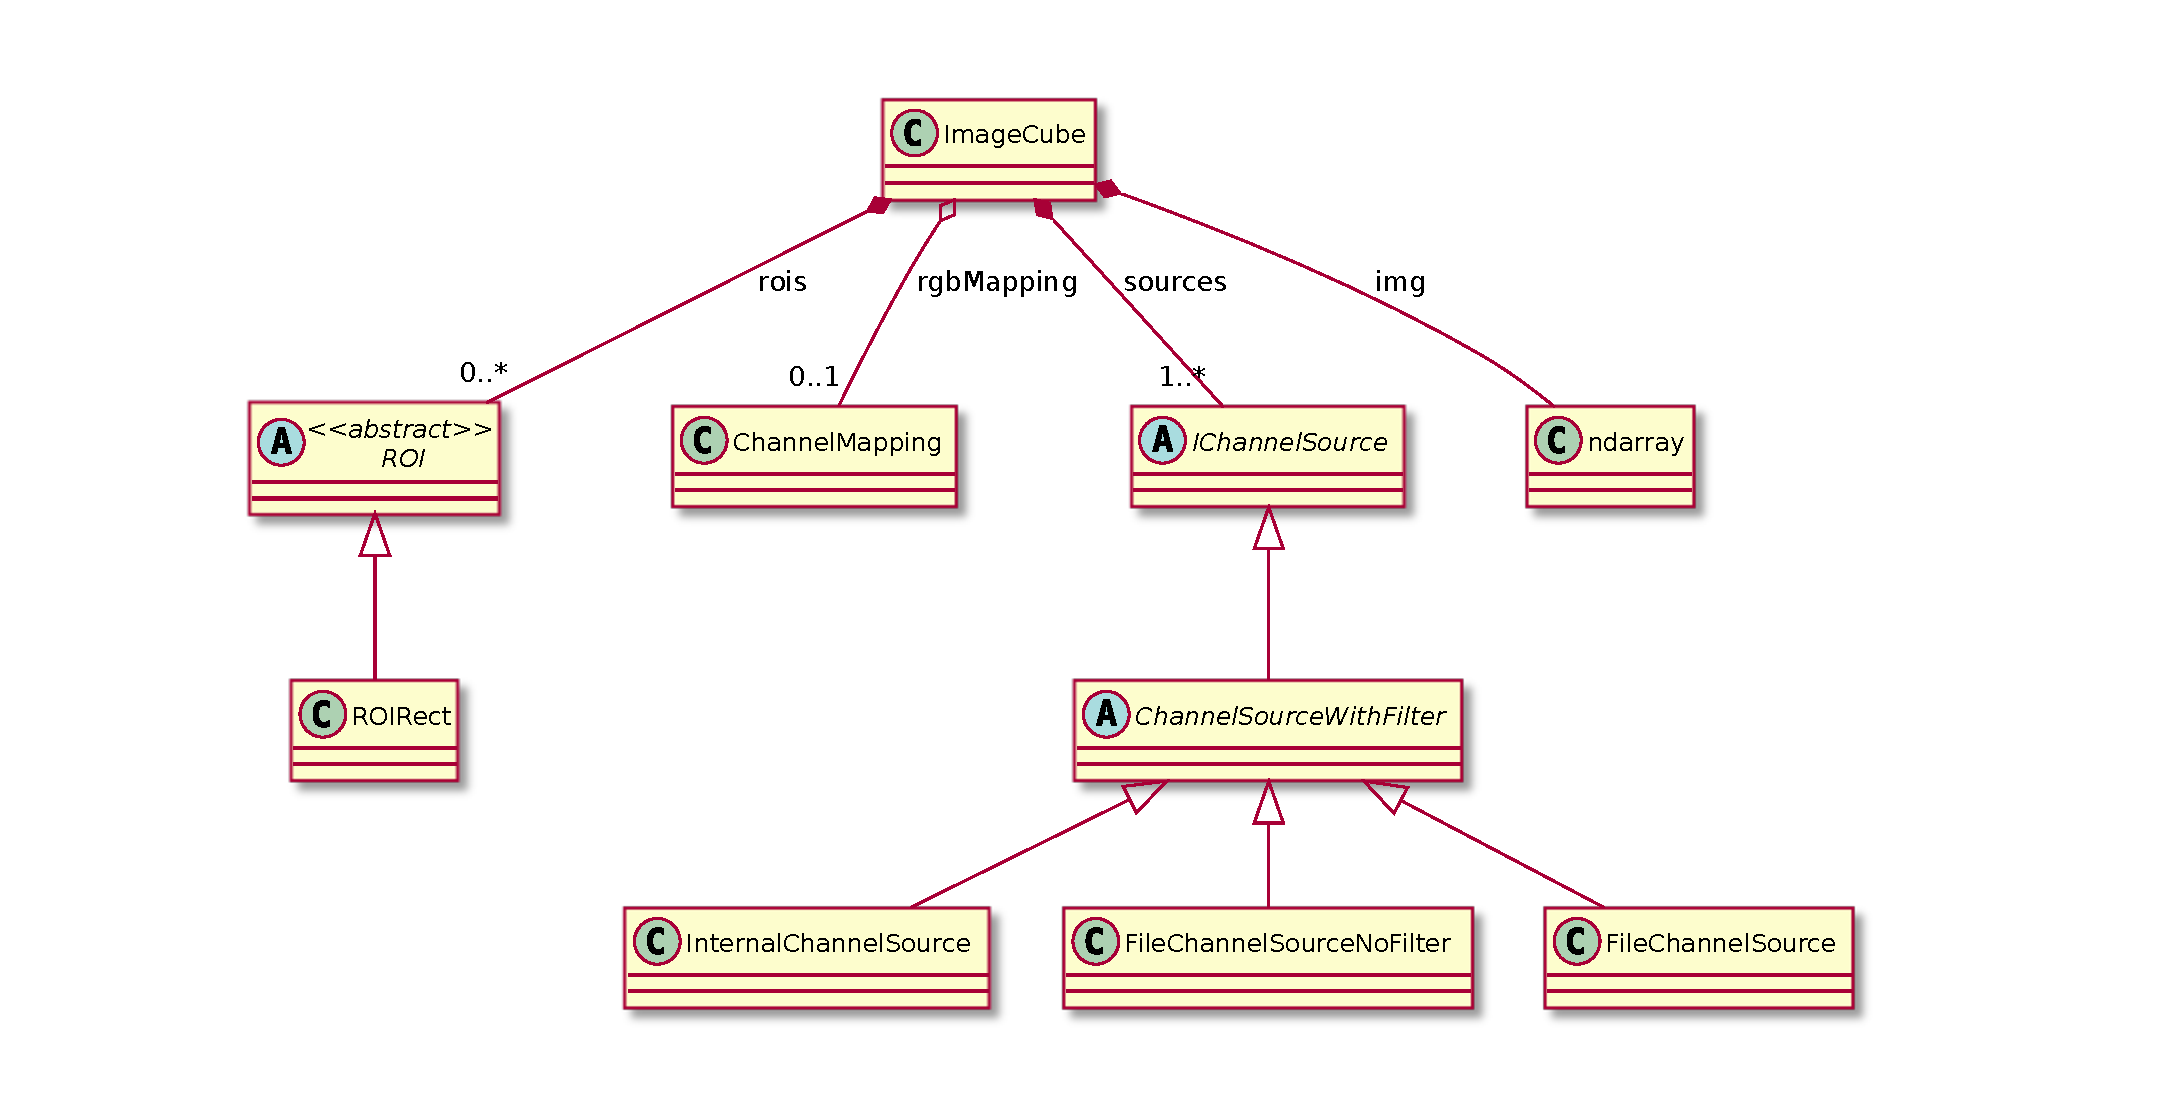
\includegraphics[width=6.5in]{image.pdf}
\caption{Outline UML class diagram of image model}
\label{image.pdf}
\end{figure}

The main class is \texttt{ImageCube}: this encapsulates a numpy array
\texttt{img}
which is the actual image data cube. This is either a 
$w \times h \times depth$ array for genuine cubes with multiple channels,
or a $w \times h$ array for a single channel image. The data type is 32-bit floating
point, and images are typically normalized to the range [0,1].

\begin{notebox}
In this document I have a tendency to refer to image data as both ``image'' and ``image cube.''
Both terms refer to the same thing: an array of floating point image data, with 1 or more channels
of information. There is no upper limit on the number of channels in an image (or image cube)
beyond system memory.
\end{notebox}


\subsubsection{IChannelSource and its implementations}
Each \texttt{ImageCube} has a number of channels, and for each channel there must be a corresponding
entry in its \texttt{sources} list. This describes where that channel came from, so that (typically) filter
information can be preserved, where appropriate, through the graph. The sources for each channel are a set
of \texttt{IChannelSource} objects. For example, if an image was loaded through the RGB loader, it might
have three ``fake'' channel sources for red, green and blue. Thus the sources will be 
\begin{v}
[ {RED}, {GREEN}, {BLUE} ]
\end{v}
i.e.\ a list of three sets, each with a single source.
If the image is then converted to greyscale, this could
become
\begin{v}
[ {RED,GREEN,BLUE}, {RED,GREEN,BLUE}, {RED,GREEN,BLUE} ]
\end{v}
because each channel now contains information from the red, green and blue channels in the source file.
The \texttt{RED}, \texttt{GREEN} and \texttt{BLUE} values refer in this case to \texttt{FileChannelSourceNoFilter} objects
which contain ``fake'' filter information and a filename identifier.
Each \texttt{IChannelSource} contains methods for accessing:
\begin{itemize}
\item an \textbf{identifier string} for the source from which the channel was acquired (typically a filename or data ID);
\item a \textbf{filter} and methods for obtaining the filter name, filter position and an actual filter reference (for extra data such as centre wavelength) (note
that much of this information will be ``fake'' for images loaded from plain RGB files);
\item methods for getting string descriptors for this source.
\end{itemize}

Nodes generate and process this information in different ways. For example, a \emph{gradient} node takes a single channel and converts it into an RGB image with
a colour gradient: here, the output image's sources are ``internal RGB'' sources with no identifier or sensible filter data because the output's colour
is entirely artificial. In contrast, a the \emph{curve} for performing a sigmoid function on all channels of an image will give the output image the
same sources as the input image.

Sources are used to keep track of each channel as it moves through the graph so they can be processed and displayed appropriately:
Fig.~\ref{app.png} shows a typical node in the ``node controls and output'' section. This section, as it does in many nodes,
contains a ``canvas'' displaying an image. Above the canvas are three combo boxes which select the channels in the image cube to display on the canvas,
and these are typically labelled by a string generated from the source data for each channel (along with the index). Sources are also used
to select channels to combine and manipulate in those nodes which do so.

\subsubsection{RGB channel mappings}
The previous section briefly mentions the three RGB mapping combo boxes at the
top of the canvas component in the node controls in Fig~\ref{app.png}. In
canvases --- components which display images --- a multi-channel image cube
must be displayed as RGB data. The combo boxes control how this is done, and
the data is made persistent in a slightly complicated way, as shown in Fig.~\ref{rgb.pdf}.

\begin{figure}[ht]
\center
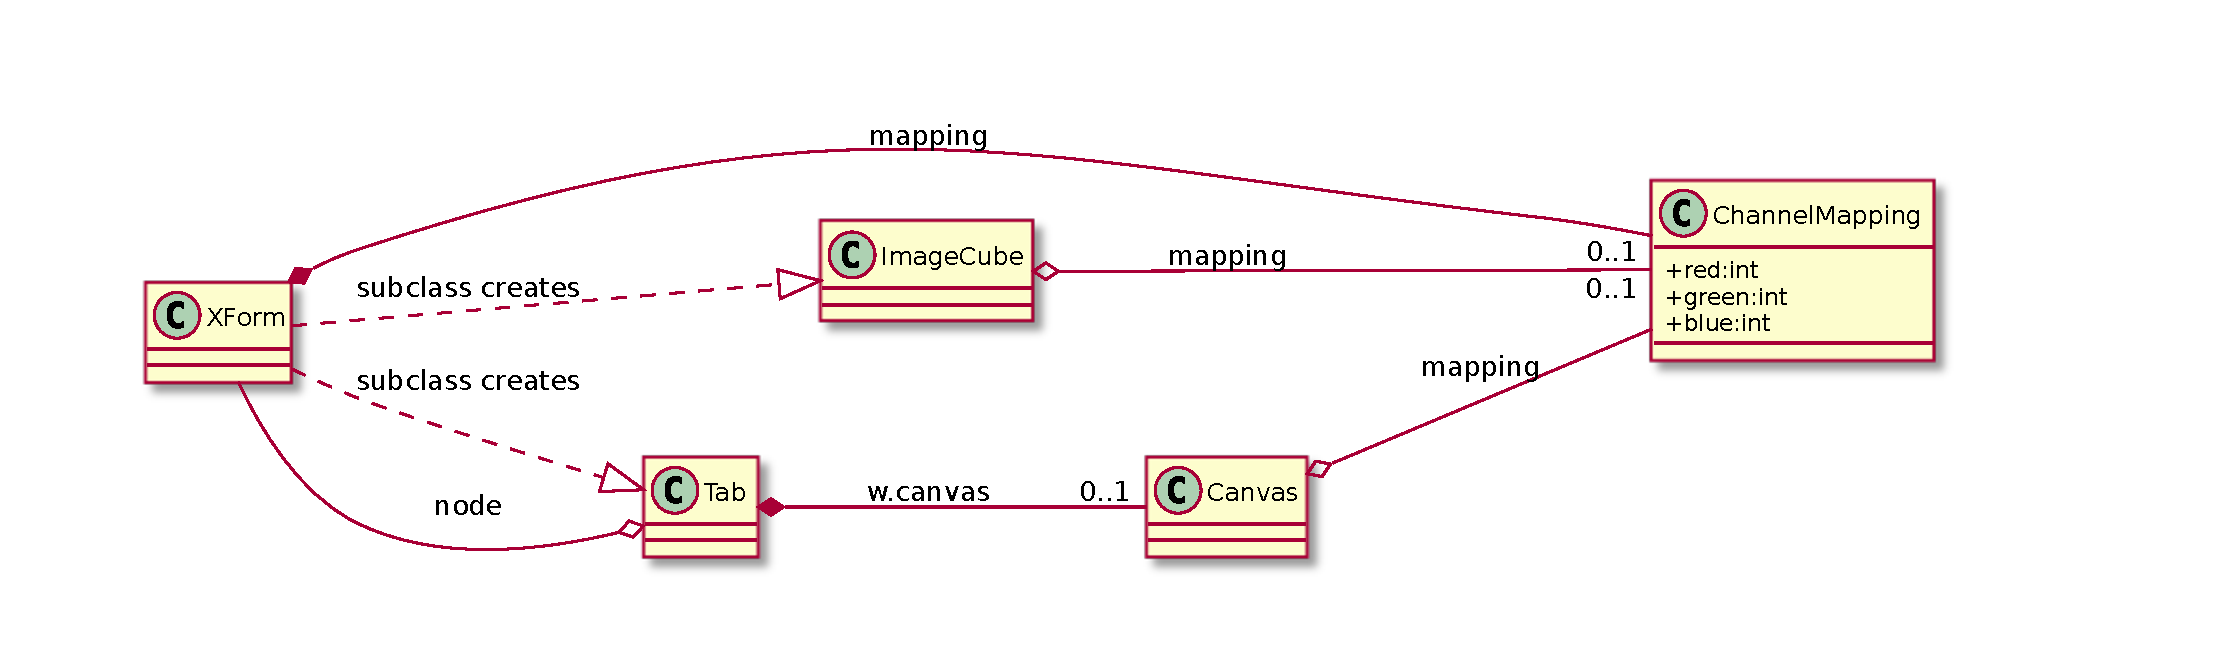
\includegraphics[width=6in]{rgb.pdf}
\caption{RGB mapping classes}
\label{rgb.pdf}
\end{figure}

The relationships will hopefully become clearer when I come to describe how nodes work in more
detail, but for now:
\begin{itemize}
\item A \texttt{ChannelMapping} object consists of three integers giving the indices of 
the channels in an image cube to display in the red, green and blue channels on screen.
\item An \texttt{XForm} (i.e.\ a node) may need to show an image on a canvas. If so, it 
will use the \texttt{mapping} field in \texttt{XForm} to store a mapping. This is provided
as a convenience, not all node classes will use it. Some may need to create more if they 
display more than one image.
\item When an \texttt{XForm} creates an image for display or passes
one through, it sets the mapping of the image to the mapping of the node. This is used in the
\texttt{rgb()} method to generate the RGB representation.
\item When an \texttt{XForm} is opened for modification, it creates a subclass of \texttt{Tab}.
This will contain a \texttt{Canvas}, which is given a reference to the mapping inside the
\texttt{XForm}. It needs this so that the mapping can be modified even when no image is present.
\end{itemize}
This may seem rather redundant, but
\begin{itemize}
\item The mapping must be be owned by the node, so it can be serialised and persists when
there is no image and no open tab.
\item We must have a reference to the mapping in the canvas, so it can be manipulated by
the combo boxes even when no image is present.
\item Finally, we need a reference to the mapping in the image so that \texttt{rgb()} can be called
on the image when it is input into another node. This is used in nodes like \emph{inset}, which
operate entirely on RGB representations --- it's much neater if these are the RGB representations
output by the nodes which feed in.
\end{itemize}
A few nodes have an extra complication --- they may output an RGB representation. In this case, the RGB conversion
needs to be done inside the node itself for output, rather than inside the canvas solely for display. A good node
to study for details on how to do this is \emph{rect}. In essence, the Canvas is told to display the ``premapped''
RGB image generated inside the node's \texttt{perform()} method. It is also given a node reference so that
the node can be performed again (thus regenerating the RGB image) whenever a mapping combo box is changed.

\subsubsection{Regions of interest}
Regions of interest belong to images, and modify how nodes process those
images. They are added to images by region of interest nodes such as
\emph{rect}. Figs.~\ref{app.png} and \ref{graph.png} show this in action:
\begin{itemize}
\item A file is read in, producing an image cube
\item A \emph{rect} node adds a region of interest to this image. The outputs are:
\begin{itemize}
\item the image with the rectangle added to its list of ROIs;
\item the image cropped to the bounding box of the list of ROIs (at the moment, just this rectangle)'
\item an RGB representation of the image (according to the previous node's canvas RGB mapping);
annotated with the rectangle and some text, and also an ROI added describing the rectangle;
\item the rectangle datum itself.
\end{itemize}
\item a \emph{decorr stretch} takes the annotated RGB representation output and imposes a decorrelation
stretch --- but only on the regions of interest in the image (in this case, inside the rectangle)
\item a \emph{histequal} node performs a histogram equalisation, again honouring the regions of interest
which have been passed through the previous node unchanged.
\end{itemize}
As shown in Fig.~\ref{image.pdf}, each image contains a list of \texttt{ROI} objects,
each of which is an instantiation of a subclass of \texttt{ROI}. 

To honouring regions of interest inside a node's \texttt{perform()} method:
\begin{itemize}
\item \texttt{ImageCube.subimage()} will return a \texttt{SubImageCubeROI} object. This encapsulates
a numpy array containing the image bounded to a rectangle around the regions of interest and
a boolean mask (again as a numpy array) specifying which pixels in this rectangle are actually
in regions of interest.
\item The manipulation can now be performed on the \texttt{img} field of this ``subimage,'' but
only on those pixels whose values are true in the corresponding \texttt{mask} field.
\item The modified pixels can be ``spliced'' into the original image cube, creating a new image
cube, using the \texttt{modifyWithSub} method.
\end{itemize}
This example shows the operation of the decorrelation stretch:
\begin{lstlisting}[language=Python]
    def perform(self,node):
        img = node.getInput(0)
        if img is None:
            node.img = None
        elif not node.enabled:
            node.img = img
        elif img.channels != 3:
            ui.error("Can't decorr stretch images with other than 3 channels")
        else:
            subimage = img.subimage()
            newimg = decorrstretch(subimage.img, subimage.mask)
            node.img = img.modifyWithSub(subimage, newimg)
        if node.img is not None:
            node.img.setMapping(node.mapping)
        node.setOutput(0, node.img)
\end{lstlisting}
There are several checks for whether the node is actually enabled, and whether there is an image
present to stretch, but the core lines are these:
\begin{lstlisting}[language=Python]
            subimage = img.subimage()
            newimg = decorrstretch(subimage.img, subimage.mask)
            node.img = img.modifyWithSub(subimage, newimg)
\end{lstlisting}
The \texttt{decorrstretch} takes two arguments: the numpy array containing the pixels which bound
the ROIs, and the mask for those pixels in that array which are in the ROIs. It returns an image
of the same size, which is then spliced back into the original image. The new image returned
will have the same channel sources, the same ROIs and the same RGB mapping.

\begin{notebox}
Much of the ROI system is work in progress, particularly combining
multiple ROIs. This documentation might change.
\end{notebox}


\subsection{Macros}
\label{macros}
Macros are one of the more complex parts of the PCOT data model, so it's
important that they are documented here. First, a quick description
of how they work from a user standpoint.

Users can create a new macro, which will open a window with a new graph in it.
This is distinguished from the main window by its slightly different
background colour. The user can create and manipulate transform nodes inside
this graph, as usual. This is the \textbf{prototype graph} for the macro.
The user should create special input and output nodes inside this graph
to allow data to flow into and out of the macro.

When a new macro is created, a button for that macro appears in the ``palette''
on the right of the app window. Clicking on this button will create
an \textbf{instance} of the macro inside the main graph. This is a
node which contains a copy of the prototype graph --- it must be a copy,
because multiple instances of the macro with different data may exist.
When the user edits the prototype graph (including the parameters of 
any nodes within it) the changes are copied to the instance graphs for
that macro. Thus the user now has a single graph which can be changed,
which represents a set of nodes inside a single node. Multiple instances
of the macro can be made which will all share the same parameters.

\subsubsection{Macro internals}
Each macro node contains an instance graph copied from the prototype
graph, which has a set of components interfacing between the instance
graph and the graph in which the instance is embedded.
Consider the situation in Fig.~\ref{macroobjs.pdf}.
\begin{figure}[ht]
\center
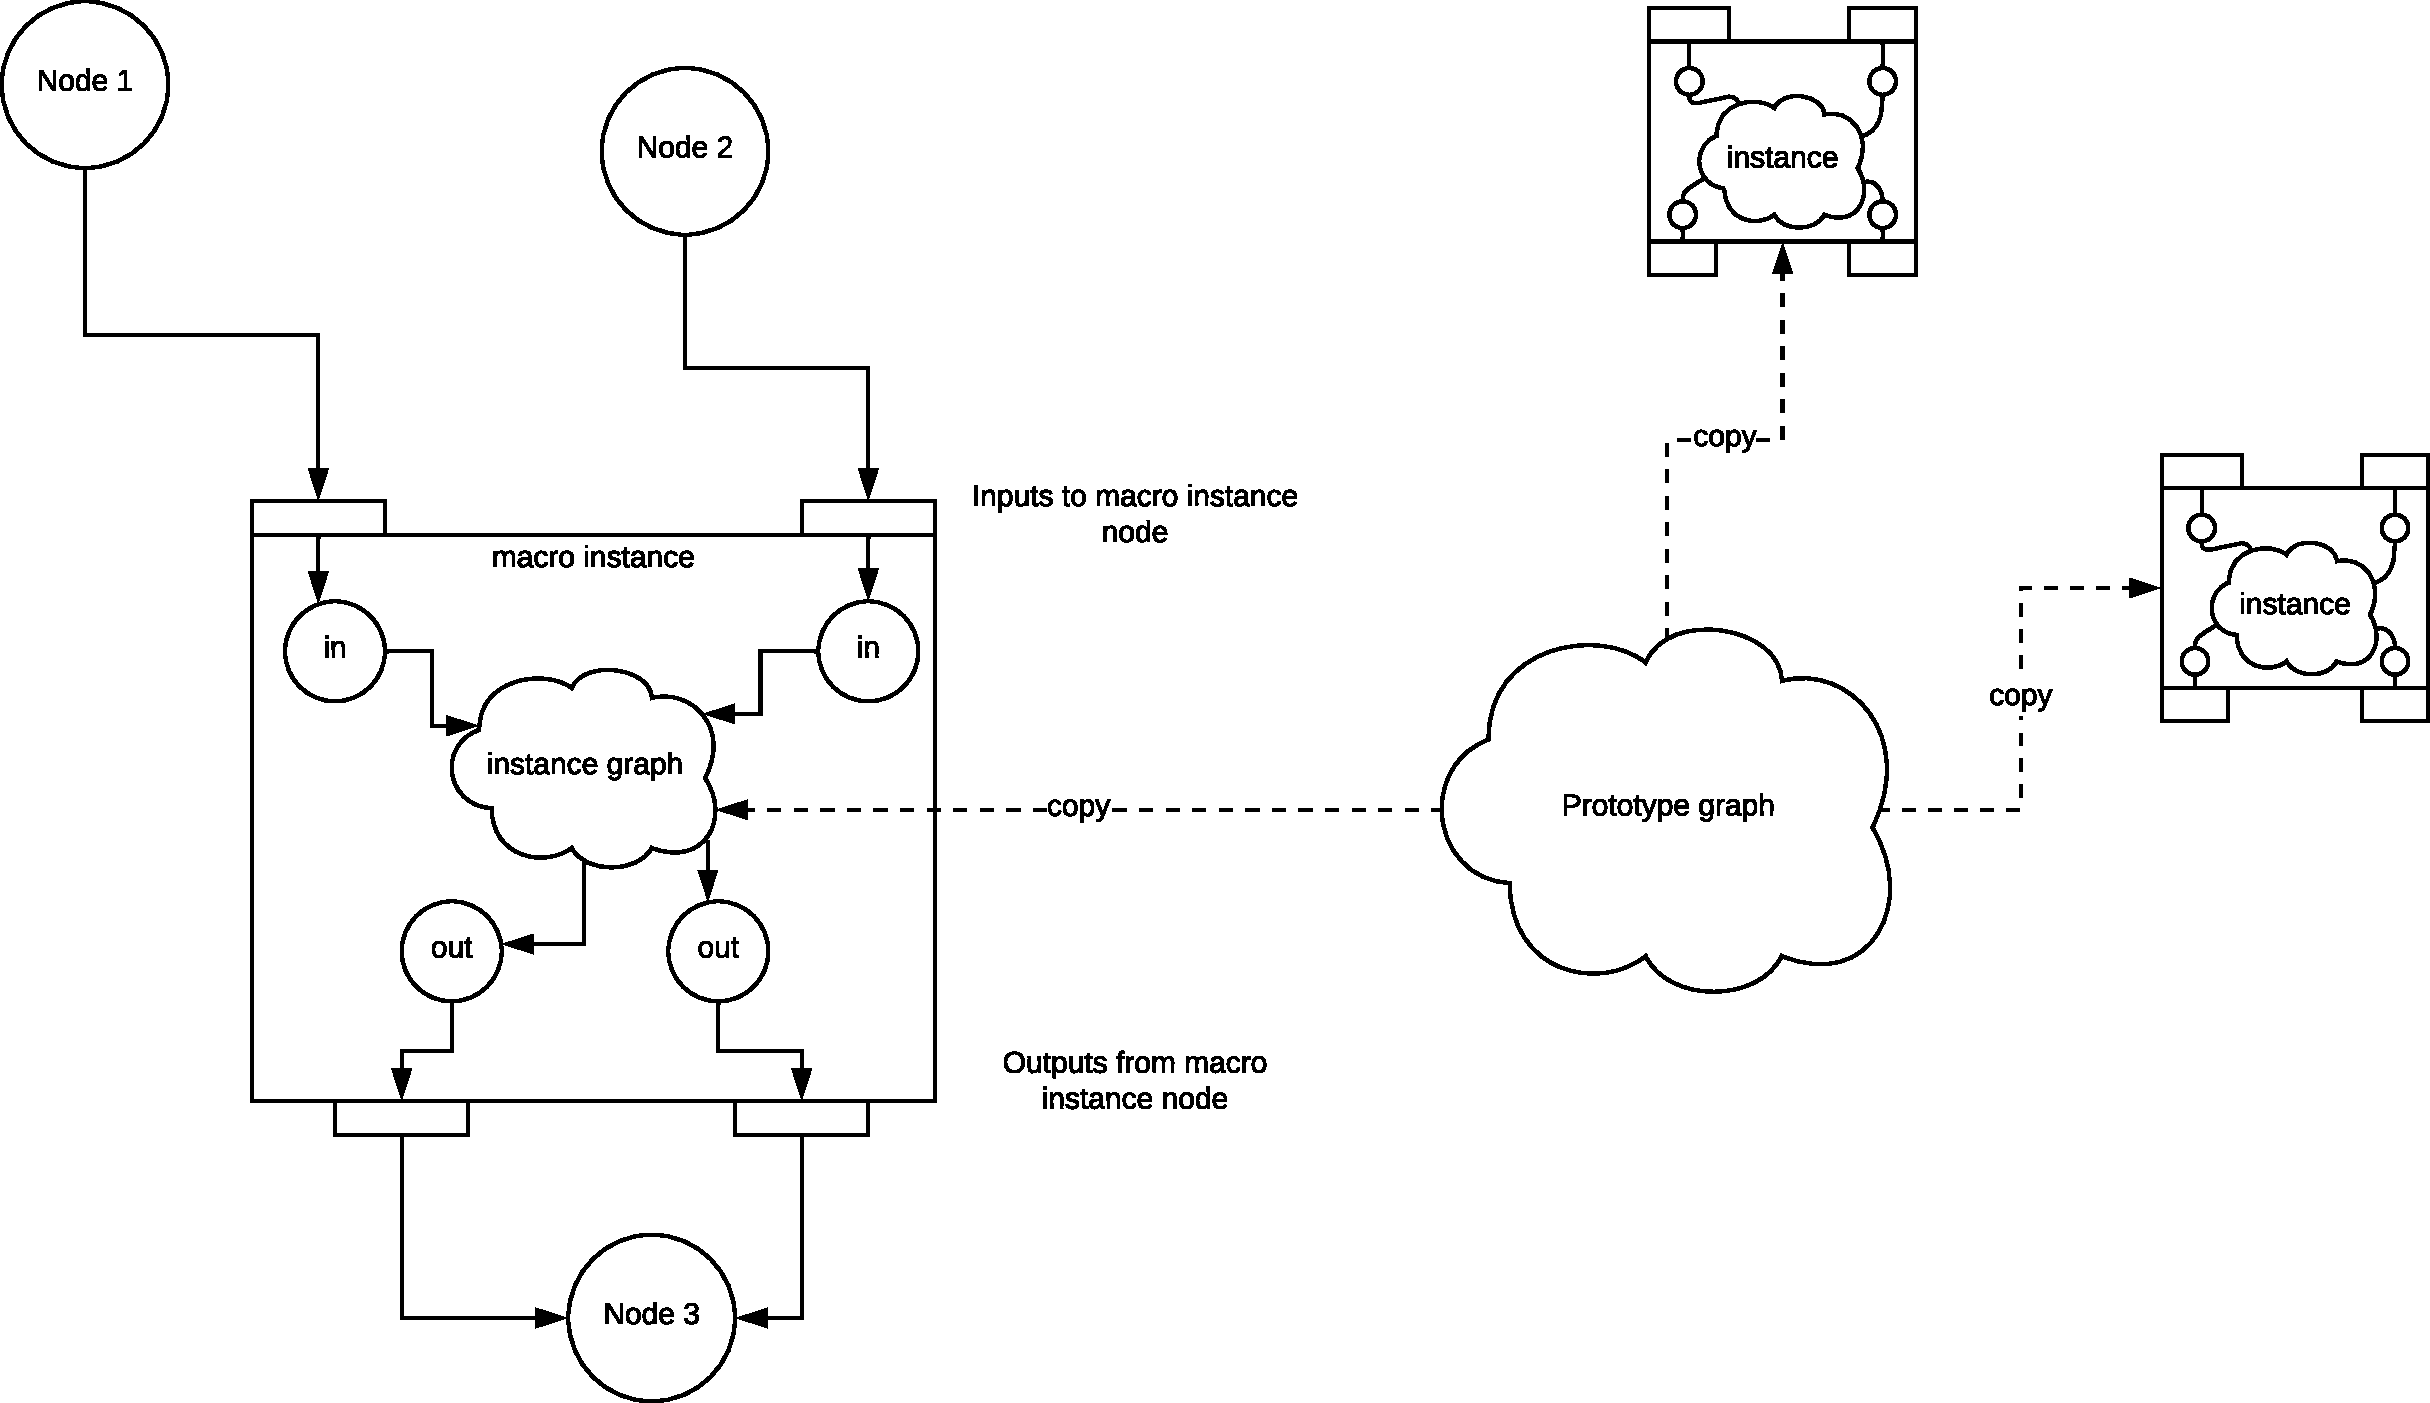
\includegraphics[width=5in]{macroobjs.pdf}
\caption{An example of a graph containing macros}
\label{macroobjs.pdf}
\end{figure}
This contains three instance nodes of a single macro. 
I have ``zoomed in'' on one of the instances, showing that it is connected
to three other nodes: two on its inputs, one on its outputs.
When this main graph runs, the following happens:
\begin{itemize}
\item Node 1 is able to run, does so, and sets its output
\item The macro instance cannot yet run
\item Node 2 is able to run, does so, and sets its output
\item The macro instance can now run:
\begin{itemize}
\item The macro instance node copies its input data
into the input nodes contained within the instance graph
\item The input nodes in the instance graph are run
\item The nodes dependent on those input nodes are run (i.e.\ the
instance graph proper)
\item The output nodes in the instance graph are run, copying their
inputs into the macro instance node's outputs
\item the instance now has now completed its run
\end{itemize}
\item Node 3 can now run, reading its inputs from the macro instance node.
\end{itemize}

\subsubsection{Macro inefficiencies}
\label{macroineff}
As noted above in Sec.~\ref{graphperform}, all the nodes in all instance
graphs are run whenever the prototype graph is changed. This is very
inefficient and may cause considerable delays. It's done by simply forcing all
\texttt{XFormMacro} nodes which are instances of the macro to perform themselves. Here
is the relevant part of \texttt{XFormGraph.changed()}:
\begin{lstlisting}
    # distribute changes in macro prototype to instances.
    # what we do here is go through all instances of the macro. 
    # We copy the changed prototype to the instances, then run
    # the instances in the graphs which contain them (usually the
    # main graph).
    # This could be optimised to run only the relevant (changed) component
    # within the macro, but that's very hairy.

    for inst in self.proto.instances:
        inst.instance.copyProto()
        inst.graph.performNodes(inst)
\end{lstlisting}
Here, \texttt{inst} is each \texttt{XFormMacro} node inside the main graph. Thus
\texttt{inst.graph} will be the main graph (for an non-nested macro). The
\texttt{self} value is the macro prototype graph, because this
method was called on an object inside that graph. This code therefore calls
\texttt{performNodes()} on the main graph to run the \texttt{XFormMacro} node inside
that graph. 

In an ideal world, this process --- calling \texttt{changed()} --- would identify
the instance node which corresponds to the prototype node which was changed, and only
run that inside the instance graph for the macro. The child nodes of the instance node
would then need to be run.


\subsection{User interface}
The user interface is mainly in the \texttt{ui} package, although each
node type's file contains its UI code (a subclass of \texttt{ui.tabs.Tab}.
A reasonably full view of the system is shown as a class diagram
in Fig.~\ref{ui.pdf}.
The main files involved are:
\begin{itemize}
\item \texttt{ui/mainwindow.py}: the main window classes;
\item \texttt{ui/tabs.py}: the \texttt{DocktableTabWindow} and \texttt{Tab}
classes (also the \texttt{ExpandedTab} class for when a tab is undocked);
\item \texttt{ui/canvas.py}: the Canvas widget for viewing image cube slices;
\item \texttt{graphview.py}: contains \texttt{GraphView}, the
\texttt{QGraphicsView} subclass which encapulates a view on the graph scene;
\item \texttt{graphscene.py}: contains \texttt{XFormGraphScene},
the \texttt{QGraphicsScene} subclass which contains a set of 2D objects
representing an \texttt{XFormGraph} and its nodes. It also contains the
classes representing those 2D objects (subclasses of various Qt graphics item
classes).
\end{itemize}

\begin{figure}[ht]
\center
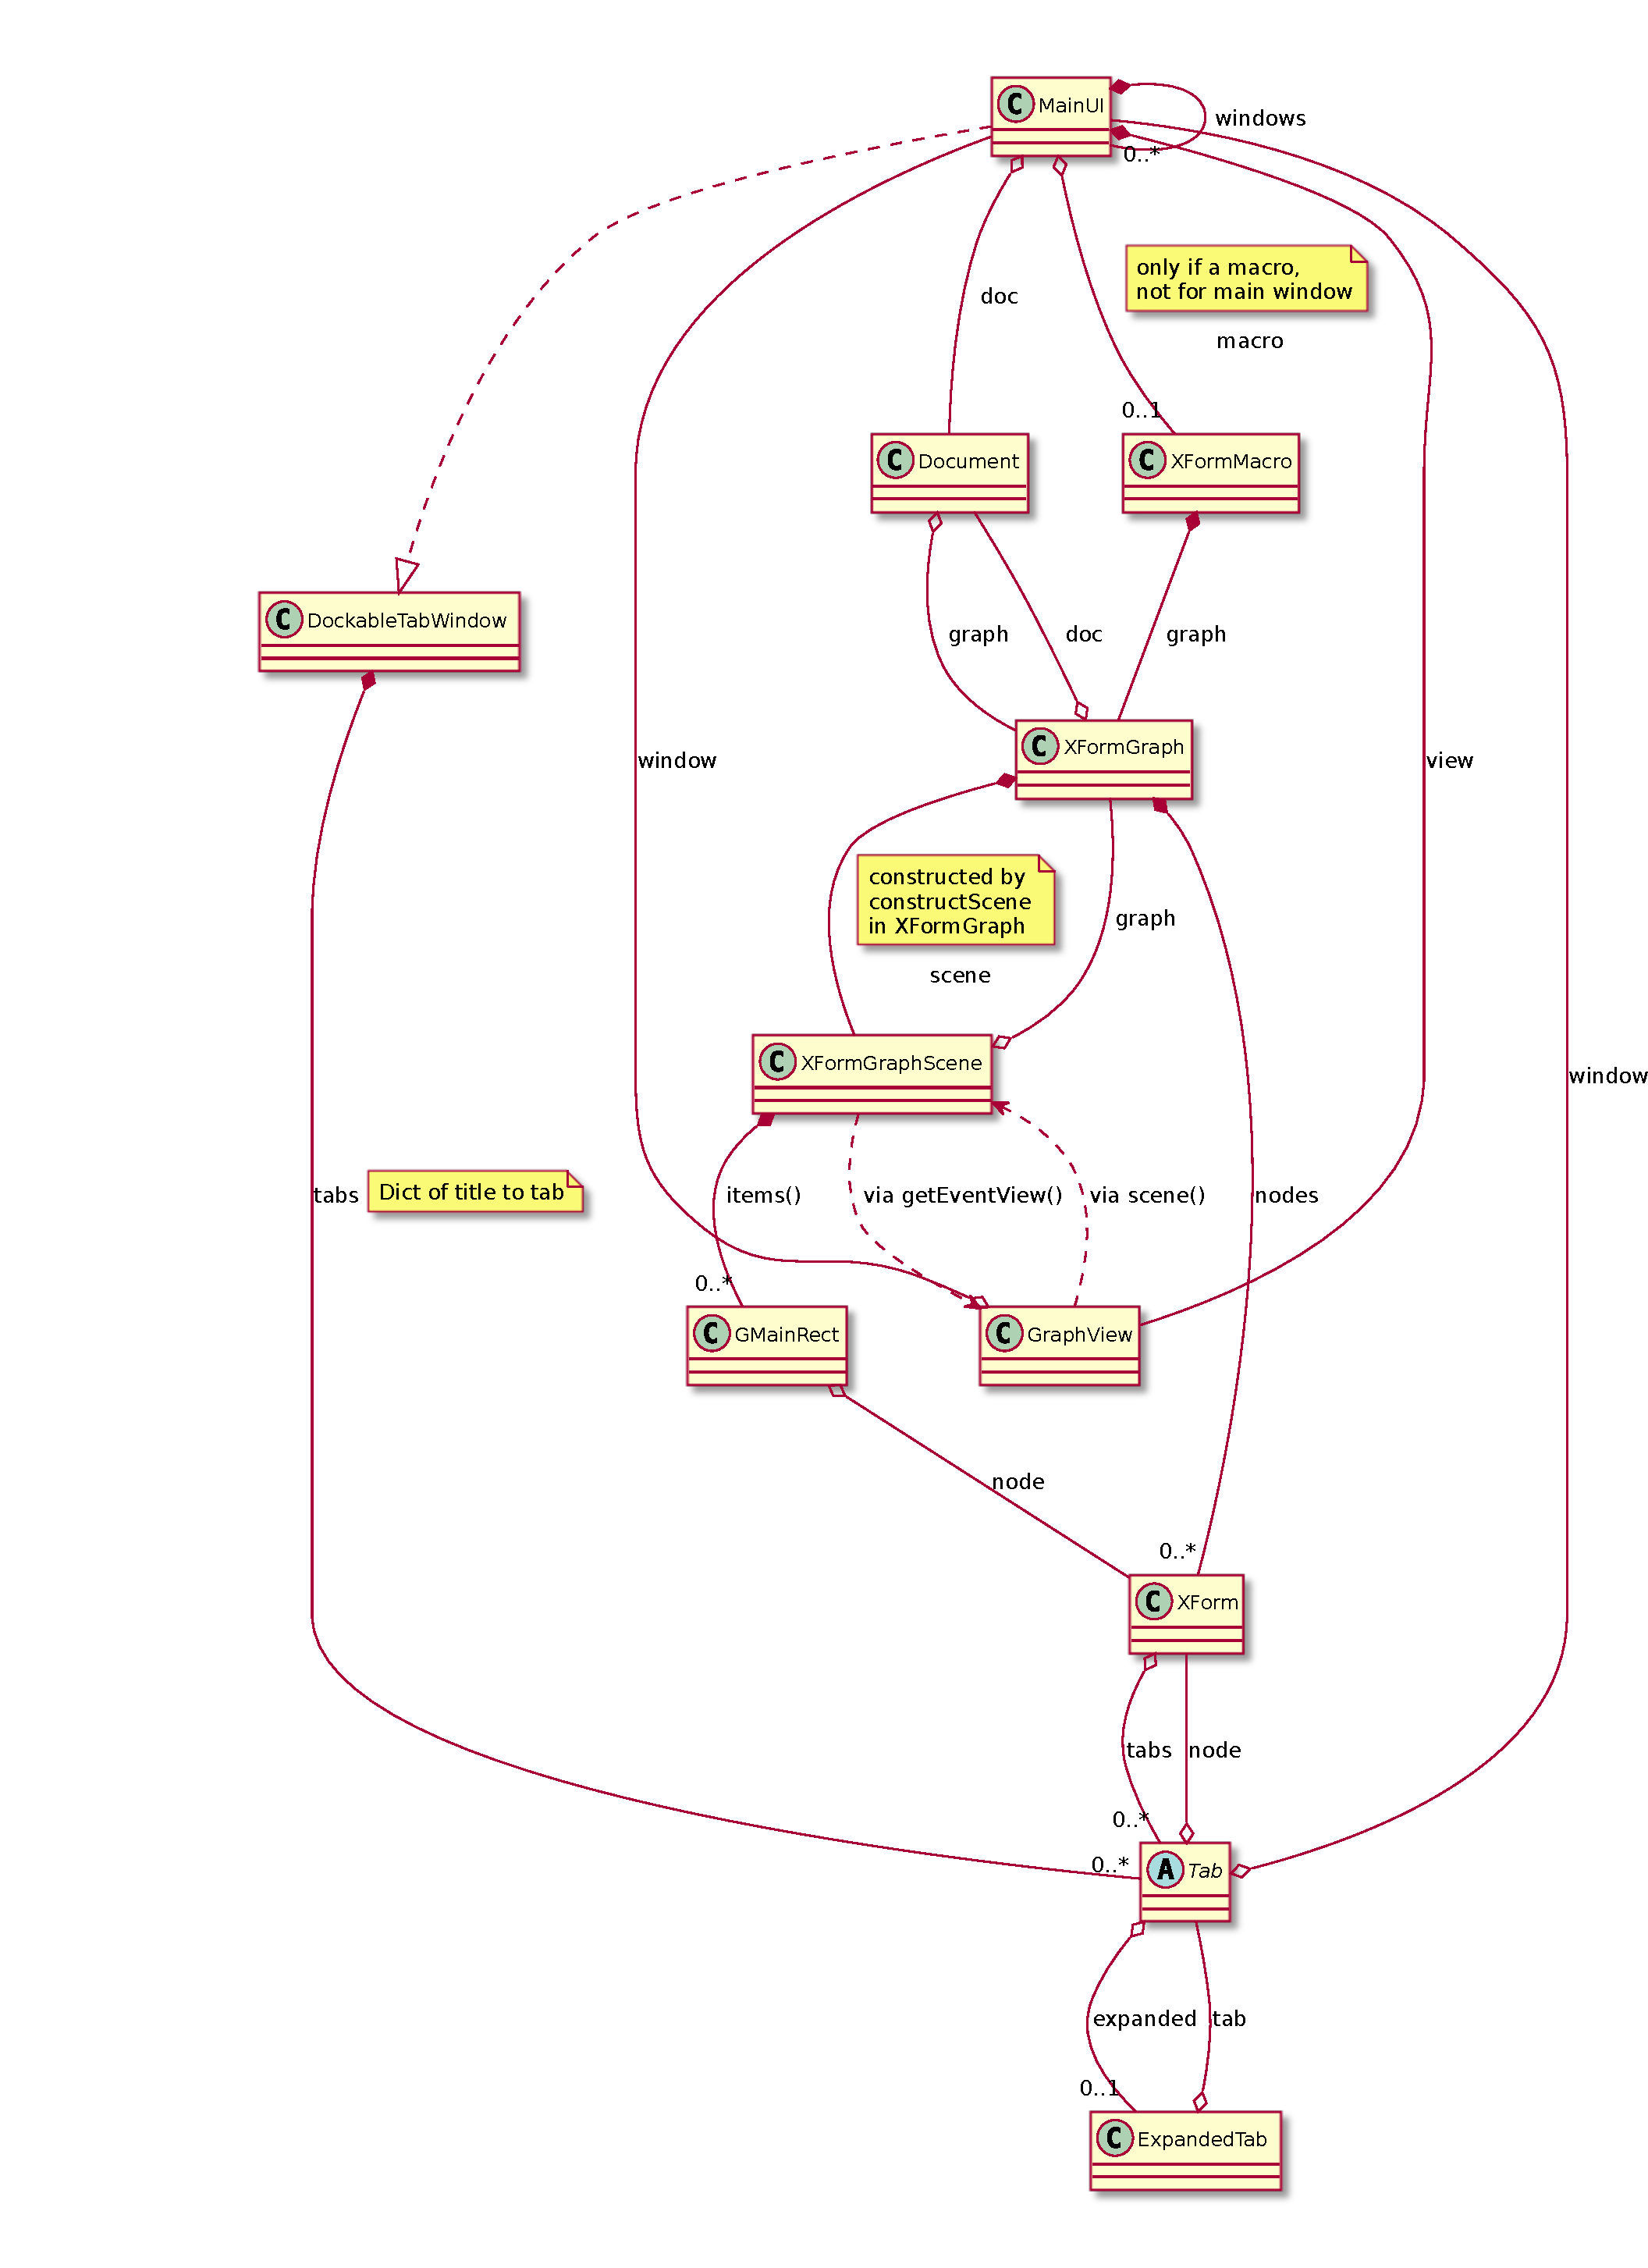
\includegraphics[width=4in]{ui.pdf}
\caption{UI class diagram}
\label{ui.pdf}
\end{figure}


\clearpage
\subsubsection{The main window}
The main window class is \texttt{ui.mainwindow.MainUI}. They contain the
following main widgets:
\begin{itemize}
\item a \texttt{QTabWidget} to hold the dockable tabs (tab docking is
handled by the \texttt{DocktableTab} superclass);
\item a \texttt{GraphView} widget to manage viewing and manipulating
the graph;
\item a \texttt{Palette} to contain the buttons to create new nodes
\end{itemize}
The bottom pane contains various widgets, such as the log console and
caption control combo box.
Main windows are created:
\begin{itemize}
\item when the application opens the first empty main graph in \texttt{main.py}
\item when a new, empty main graph window is created
\item when a window for a macro prototype graph is created
via \texttt{createMacroWindow()}.
\end{itemize}
There are some ownership oddities here. In the first two cases
the \texttt{MainUI} constructor is called with no arguments. This will
cause it to create a new \texttt{XFormGraph} which the window will own.
In the last case, the constructor is informed that the graph is a macro
prototype. This causes the UI to be created slightly differently. 
The \texttt{createMacroWindow()} static method then sets the graph to the macro's
prototype, which is owned by the \texttt{XFormMacro}.

In both cases, the \texttt{XFormGraphScene} contains a Qt Graphics Scene
which is constructed and regularly updated from the graph (by calling
its \texttt{rebuild()} method). This is viewed in
the main window through the \texttt{GraphView} class. Both these classes
accept various user actions and use them to modify the graph.


% Created by Jim Finnis
% Date Wed Mar 3 15:15:17 2021


\section{Anatomy of an \texttt{XForm}: how to write nodes}
As noted above and shown in Fig.~\ref{xform.pdf}, all nodes are 
implemented as subclasses of \texttt{XFormType}. Each node 
is an \texttt{XForm} with a link to an \texttt{XFormType} object
controlling its behaviour\footnote{an example of ``favouring
composition over inheritance.''}.
There is only one object of each \texttt{XFormType} class; they
are singletons. The data differentiating each instance of 
a given node type is stored in the \texttt{XForm} itself.

To write a new node type we need to write a new \texttt{XFormType},
create a singleton object of that class, and register it with the system
(so the user can see it). The last two steps are dealt with automatically;
all we need do is write the class inside the \texttt{xforms} directory
and make sure it has the \texttt{@xformtype} annotation to ensure
it is registered and is a singleton, as described in 
Sec.~\ref{xformtype}.

In addition to an \texttt{XFormType}, it may be necessary to write
a subclass of \texttt{ui.tabs.Tab} to display its controls and output.
If the new node only displays
an image and has no extra controls, the built-in \texttt{TabImage}
can be used: I will discuss this case first.

\subsection{An example}
The required methods are described in Sec.~\ref{xformtype}. This
section will give an example of how to build an image manipulation
node --- an image normalisation node, which will normalise all channels
to the range [0,1]. It will also honour regions of interest:
only pixels inside the currently active ROI will be processed. This makes
image processing a little more complicated.

\subsubsection{Writing the operation}
We will be working in a file inside the \texttt{xforms} directory, which is
imported by \texttt{main.py}. We'll call this file \texttt{xformnorm.py}.
First, we need to write a function to normalise the image as a 3D numpy array,
taking into account a boolean mask of pixels to ignore (for the region
of interest). The declaration is simple:
\begin{lstlisting}
def norm(img, mask):
\end{lstlisting}
Now we need to generate a numpy masked array from the image and mask.
Note that the mask passed in uses True to indicate array elements which should
be used --- this is intuitively more obvious, but the construction
of a masked array uses True to indicate elements which are masked out. Thus
we need to negate the mask:
\begin{lstlisting}
    masked = np.ma.masked_array(img, mask=~mask)
\end{lstlisting}
Now we need to create a copy of the array to write the data to because we
don't want to modify the original image:
\begin{lstlisting}
    cp = img.copy()
\end{lstlisting}
Next we want to find the minimum and maximum of the pixels in the masked
image (i.e.\ ignoring unmasked pixels):
\begin{lstlisting}
    mn = masked.min()
    mx = masked.max()
\end{lstlisting}
If the range is zero, we generate an error --- we'll return this and deal
with it in \texttt{perform()}, our node's actual work function. We also
generate a zero image as the result.
If the range is OK, the exception is None and the result image is
the input image normalised
to the range of the masked pixels:
\begin{lstlisting}
    if mn == mx:
        ex = XFormException("DATA", "cannot normalize, image is a single value")
        res = np.zeros(img.shape,np.float32)
    else:
        ex = None
        res = (masked - mn) / (mx - mn)
\end{lstlisting}
We now put the result image into the image copy we generated earlier,
but this time we don't negate the mask (because \texttt{putmask} works
the right way --- pixels which are True in the mask are written). We 
then return the exception and the modified image copy.
\begin{lstlisting}
    np.putmask(cp, mask, res)
    return ex, cp
\end{lstlisting}
As you can see, error handling and dealing with regions of interest
is often the most complicated part of a node!
Now we can start to write the actual node class.
\subsubsection{The \texttt{XFormType} subclass}
As described above in Sec.~\ref{xformtype}, the behaviour of an \texttt{XForm} node is determined
by the \texttt{XFormType} singleton to which it is linked. The code for this class will start like this:
\begin{lstlisting}
@xformtype
class XformNormImage(XFormType):
\end{lstlisting}
We're creating a new subclass of \texttt{XFormType} and giving it the
\texttt{@xformtype} annotation, which will create an instance and register it
automatically with the application. Because of this, the declaration is the
only place where the name of the class is used. Now the constructor:
\begin{lstlisting}
    def __init__(self):
        super().__init__("normimage", "processing", "0.0.0")
        self.addInputConnector("", conntypes.IMG)
        self.addOutputConnector("", conntypes.IMG)
        self.hasEnable = True
\end{lstlisting}
The superconstructor call sets the node name, the group under which it appears
in the palette, and a version number. The next two lines define an input and
output connector. These have optional names, which are both empty in this
example. This is the usual approach: names are only used to annotate the nodes
in the graph, and are left empty where they are obvious. In the code,
connectors are referenced by index in order of creation. Both connectors here
are images, with type \texttt{IMG}. See \texttt{conntypes.py} for all the
types. The final line sets the node to have an \texttt{enabled} value and
associated toggle button. This is used in nodes which may be computationally
intensive, to temporarily ``turn them off.'' This will usually be handled by
passing through the data unchanged.

The next method is \texttt{createTab()}, which is used to create a tab for a particular node. Like most
methods in this class, it takes a reference to the node. It also takes a reference to the main window
in which the tab should be created:
\begin{lstlisting}
    def createTab(self, n, w):
        return TabImage(n, w)
\end{lstlisting}
In this class, we are using the built-in \texttt{TabImage} tab which has a single canvas widget
displaying an image. Many node types use this.

The \texttt{init()} method is used to initialise an \texttt{XForm} node to be a
particular class (beyond setting the \texttt{type} field, which is done
elsewhere). It therefore takes a node, and typically sets up private data
this type requires inside the node object. This uses an advantage of
Python\footnote{Although from a software engineering point of view it is also
a weakness.}: we can add fields to objects after they have been instantiated.
Here we just add a \texttt{img} field to store the normalised image,
initialising it to None (the
canvas widget will display a None image as a blue empty rectangle):
\begin{lstlisting}
    def init(self, node):
        node.img = None
\end{lstlisting}

\subsubsection{Writing the perform method in full}
Finally we come to the \texttt{perform()} method, which describes how this
type of node performs its operation. Here I'll describe it in full. Many
nodes, however, perform a simple operation with a few numeric parameters
on an image and output an image. These nodes can be written in a 
simpler way which also allows them to be used as functions in the 
\emph{eval} node. This will be dealt with later.

Again, it requires a reference to the
\texttt{XForm} node object which contains the node state, and its first action
is to pre-set the output image to None and then fetch the input image:
\begin{lstlisting}
    def perform(self, node):
        node.img = None    
        img = node.getInput(0, conntypes.IMG)
\end{lstlisting}
This will get a reference to the image stored in the output field of the node
connected to this node's zeroth input (the first added in the type
constructor). If there is no connection, None will be returned. None will also
be returned if the type is not \texttt{IMG}: this version of \texttt{getInput()} will
unwrap the \texttt{Datum} and type-check (see Sec.~\ref{linkage}). We then check to see if the input
is None. If it is, we do nothing (leaving \texttt{node.img} as None). We also
check to see if the node has been disabled (this node has an Enabled button):
\begin{lstlisting}
        if img is not None:
            if node.enabled:
\end{lstlisting}
Assuming these are both true, we use the \texttt{ImageCube.subimage()} method to fetch
a \texttt{SubImageCubeROI} object containing information about which parts of the image are
in the current region of interest: the rectangle of pixels bounding the region and the mask
describing which pixels within that bounding box are in the region. We can then pass these two numpy
arrays into the normalization function we wrote earlier, obtaining another numpy array: the 
bounded image normalized. We then call \texttt{modifyWithSub()}, which creates a new ImageCube
in which the section described by the region of interest (taking into account the mask)
has been replaced by the new, normalized image data:
\begin{lstlisting}
                subimage = img.subimage()
                ex, newsubimg = norm(subimage.img, subimage.fullmask())
                if ex is not None:
                    node.setError(ex)
                node.img = img.modifyWithSub(subimage, newsubimg)
\end{lstlisting}
Note the error check: our normalization function returns an exception and an
image. If the exception exists (is not None), we set the error state in the
node (see Sec~\ref{errorhandling}). It's still fine to patch in the subimage,
though. This entire process is shown in Fig.~\ref{norm.pdf}.

\begin{figure}[ht]
\center
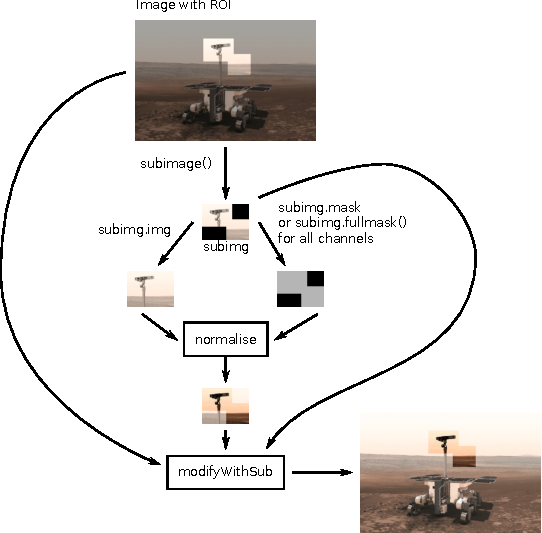
\includegraphics[width=5in]{norm.pdf}
\caption{The image processing in the norm node}
\label{norm.pdf}
\end{figure}
\clearpage
Finally, if the node was not enabled we set \texttt{node.img} (our output)
to be the input image:
\begin{lstlisting}
            else:
                node.img = img
\end{lstlisting}
and output the image to the node's zeroth (and only) output, wrapping it in
a \texttt{Datum}:
\begin{lstlisting}
        node.setOutput(0, Datum(conntypes.IMG, node.img))
\end{lstlisting}


\subsubsection{Writing the perform method using operation functions}
\begin{notebox}
For now, see \texttt{xformcurve.py} along with \texttt{operations} and its 
files.
\end{notebox}



%\bibliographystyle{plain}
%\bibliographystyle{alpha}
%\bibliography{bib}
%\printbibliography

\end{document}
